\documentclass[class=book, crop=false, oneside, 12pt]{standalone}
\usepackage{standalone}
\usepackage{../../style}
\graphicspath{{./assets/images/}}

\begin{document}

\chapter{Analisi Lessicale e Linguaggi Regolari}

\section{Introduzione}

Ora che abbiamo acquisito dei mezzi più potenti per affrontare questo corso, ribadiamo il concetto di analisi lessicale: dato il programma in ingresso, l'analisi lessicale restituisce una lista di stringhe che corrisponde alle parti del linguaggio identificate; questa lista di stringhe è nota come \emph{flusso dei token}.

Lo studio del capitolo precedente di consente di sapere come vengono generti linguaggi come il seguente:

\begin{equation*}
    \label{a^nb^n}
    \{ a^n b^n \mid n > 0 \}    
\end{equation*}

Come detto in passato, un liguaggio con questa forma può essere utilizzato, ad esempio, nel caso in cui vogliamo avere un egual numero di parentesi aperte e chiuse.
Il problema che vogliamo arrivare a risolvere è, più in generale, riconoscere se una stringa faccia parte o meno del linguaggio generato da una certa grammatica.

Ad esempio, per affrontare il problema del linguaggio \ref{a^nb^n} viene naturale l'utilizzo di una struttura di tipo stack:

\begin{enumerate}
    \item leggiamo i simboli uno alla volta e li inseriamo nel nostro stack;
    \item per ogni \(a\) che leggiamo, inseriamola nella pila;
    \item se troviamo una \(b\), allora facciamo un pop dalla pila;
    \item se ad un certo punto stiamo tentando di togliere un elemento da una pila vuota o se, finita l’analisi, rimangono ancora elementi nella pila, allora c’è qualche errore;
    \item nel caso in cui al termine dell’analisi è andato tutto liscio e abbiamo svuotato la pila, allora la parola analizzata appartiene al linguaggio \ref{a^nb^n}.
\end{enumerate} 

La precedente strategia sicuramente è ottima quando il linguaggio ha una forma simile all'esempio che abbiamo considerato. Ma consideriamo invece la grammatica che genera tutte le parole dell’alfabeto:

\begin{equation}
    \label{alfabeto}
    S \to a \mid b \mid … \mid z \mid aS \mid bS \mid … \mid zS
\end{equation}

Per riconoscere parole generate da una tale grammatica il metodo di analisi naturale è una macchina a stati come quella in figura\ref{macchina_a_stati_finiti}.

\begin{figure}
    \centering
    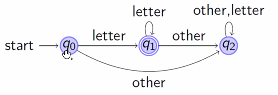
\includegraphics[width=.5\textwidth,keepaspectratio]{macchina_a_stati_finiti}
    \label{macchina_a_stati_finiti}
    \caption{Macchina a stati finiti}
\end{figure}

\noindent Il funzionamento di questi strumenti di analisi ci sarà ben più chiaro in seguito.

La grammatica che produce tutte le lettere dell’alfabeto (il linguaggio \ref{alfabeto}) è una grammatica libera, ma ha anche una caratteristica in più: è regolare. Andiamo a capire meglio di cosa si tratta.


\section{Grammatiche regolari}

Le grammatiche regolari sono un sottoinsieme delle grammatiche libere che rispettano le seguenti restrizioni rispetto alle loro produzioni:

\begin{itemize}
    \item o il body è un solo terminale (\(A \to a\));
    \item o il body è composto da un terminale e un non-terminale, nella seguente forma: \(A \to aB\);  
    \item altrimenti, il body è la parola vuota (\(A \to \varepsilon\)).
\end{itemize}

Queste grammatiche possono generare espressioni regolari, che introdurremo a breve; inoltre, i linguaggi generati da queste grammatiche sono riconosciuti dagli automi a stati finiti, sia deterministici che non deterministici.

Queste due osservazioni sono la base fondante dell'utilizzo delle grammatiche regolari per l’analisi lessicale.

\subsection{Espressioni regolari}
Prima di tutto partiamo con il definire una grammatica regolare.\\
Sia fissato un alfabeto \(\mathcal{A}\) da cui estrarre tutte le basi e sia fissato un certo numero di operatori.

Le espressioni regolari sono esprimibili tramite il meccanismo dell'induzione in questo modo.
\begin{description}
    \item[Base] Sono un'espressione regolare tutti i simboli dell’alfabeto che abbiamo scelto; in aggiunta a questi, anche \(\varepsilon\) lo è, indipendentemente dall'alfabeto scelto.
    \item[Step] Se \(r_1\) e \(r_2\) sono espressioni regolari allora:
    \begin{itemize}
        \item \(r_1 \mid r_2\) è un’espressione regolare, detta \emph{Alternation};
        \item \(r_1 \cdot r_2\) è un’espressione regolare, scritta anche come \(r_1 r_2\) e detta \emph{Concatenation};
        \item \(r_1\)\(^\ast\) è un’espressione regolare che significa ripetizione di \(r\) per un certo numero \(k\) di volte, detta \emph{Kleene star};
        \item \((r_1)\) è un’espressione regolare; è usata per definire l’ordine di svolgimento delle operazioni ed è detta \emph{Parentheses}.
    \end{itemize} 
\end{description}

\subsection{I linguaggi delle espressioni regolari}
Se un linguaggio può essere ricavato da un'espressione regolare si dice che l'espressione \emph{denota} quel linguaggio; si presti attenzione a non utilizzare il termine \emph{generare}, poiché quest'ultimo è riservato per le grammatiche generative.

Detto ciò, come capiamo qual è il linguaggio denotato da un’espressione regolare?
Consideriamo un’espressione regolare \(r\) su \(\mathcal{A}\) , il linguaggio denotato da quell'espressione \(\mathcal{L}(r)\) è anch'esso definibile tramite induzione:
\begin{description}
    \item[Base] \begin{itemize}
                    \item \(\mathcal{L}(a) = \{a\} \; \forall a \in \mathcal{A}\)
                    \item \(\mathcal{L}(\varepsilon) = \{\varepsilon\}\)
                \end{itemize}
    \item[Step] \begin{itemize}
                    \item se \(r = r_1 \mid r_2 \) \\
                    allora \(\mathcal{L}(r)= \mathcal{L}(r_1) \cup \mathcal{L}(r_2)\)
                    \item se \(r=r_1 r_2\) \\
                    allora \(\mathcal{L}(r) = \{w_1 w_2 \mid w_1 \in \mathcal{L}(r_1) \land w_2 \in \mathcal{L}(r_2)\}\)
                    \item se \(r = r_1\)\(^\ast\) \\
                    allora \( \mathcal{L}(r) = \{ \varepsilon \} \cup \{ w_1 w_2 ... w_k \mid k \ge 1 \land \forall i : 1 \le i \le k.w_i \in \mathcal{L}(r_1)\} \)
                    \item se \(r=(r_1)\) \\allora \( \mathcal{L}(r) = \mathcal{L}(r_1)\)
                \end{itemize}
\end{description}

\noindent Osserviamo ora quali sono le regole di precedenza per gli operatori appena descritti.

\begin{itemize}
    \item La Kleene star ha la precedenza maggiore;
    \item La concatenazione è seconda in ordine di precedenza;
    \item L'alternanza ha la minor precedenza.
\end{itemize}

\noindent Tutte queste operazioni hanno associatività a sinistra.
Ecco un esempio esplicativo:

\begin{equation*}
    a \mid b c^\ast
\end{equation*}

\noindent Una volta applicate le regole di precedenzam, l'espressione si legge in questo modo:

\begin{equation*}
    (a \mid ( b  ( c^\ast ) ) )
\end{equation*}    

\subsubsection{Esercizi sulle operazioni con espressioni regolari}
Ecco presentati in veloce sequenza una serie di semplici esercizi sulle operazioni con grammatiche regolari. 

\begin{itemize}
    \item \(\mathcal{L}(a \mid b) = \{a, b\}\)
    \item \(\mathcal{L}((a \mid b) (a \mid b)) = \{aa, ab, ba, bb\}\)
    \item \(\mathcal{L}(a^*) = \{a^n \mid n \ge 0\}\)
    \item \(\mathcal{L}(a \mid a^\ast b) = \{a\} \cup \{a^n b \mid n \ge 0\}\)
    \item \( (a \mid b \mid \ldots \mid z)(a \mid b \mid \ldots \mid z)^\ast \) denota l’insieme di tutte le parole dell’alfabeto
    \item \( (0 \mid 1)^\ast \) denota l’insieme di tutti i numeri binari pari
    \item \( b^\ast (abb^\ast )^\ast ( a \mid \varepsilon ) \) denota l’insieme delle parole su \(\{a,b\} \), senza alcuna occorenza consecutiva di \(a\)
    \item \( (a \mid b)^\ast aa(a \mid b)^\ast \) denota l’insieme delle parole su \( \{a,b\} \) in cui ci sono sicuramente delle occorrenze consecutive di \(a\) (date da \(aa\) in posizione centrale)
\end{itemize}

\section{Automa a stati finiti}
Gli automi a stati finiti sono usati per decidere se le parole appartengono ad un linguaggio denotato da una certa espressione regolare.
Vedremo due tipi diversi di automa a stati finiti: deterministico e non deterministico; di questi tipi poi studieremo i casidi utilizzo ottimali.

Nel caso di automa a stati finiti non deterministico i calcoli sono spesso più pesanti, perché un automa non deterministico deve vagliare più perocrsi di derivazione rispetto ai loro colleghi deterministici, i quali hanno il vantaggio di dover vagliare solo i percorsi deterministici, che sono un sottoinsieme del totale.

\subsection{Automa a stati finiti non deterministico}
Un automa a stati finiti non deterministico (NFA) è rappresentabile con una tupla
\begin{equation*}
    (S, \mathcal{A}, \textrm{move}_n, s_0, F)
    \label{nfa_tupla}
\end{equation*}
in cui:
\begin{itemize}
    \item \(S\) è un insieme di stati;
    \item \(\mathcal{A}\) è un alfabeto con \(\varepsilon \notin \mathcal{A}\);
    \item \(S_0 \in S\) è lo stato iniziale;
    \item \(F \subseteq S\) è l’insieme degli stati finali o accettabili;
    \item \(\textrm{move}_n : S \times (\mathcal{A} \cup \{\varepsilon\}) \to 2^S\) è la funzione di transizione: da un certo stato e con un certo simbolo (che può essere anche \(\varepsilon\)), mi muovo in un certo stato compreso nei sottoinsiemi di \(S\).
\end{itemize}

\subsection{Rappresentazione grafica}
La tupla \((S, \mathcal{A}, \textrm{move}_n, s_0, F)\) può essere rappresentata con un grafo diretto seguendo queste convenzioni:
\begin{itemize}
    \item gli stati rappresentano i nodi;
    \item lo stato iniziale è identificato da una freccia entrante;
    \item gli stati finali sono rappresentati da un doppio cerchio;
    \item le funzioni di transizione rappresentano gli archi, ad esempio \(\textrm{move}_n(S_1, a) = \{S_2, S_3\}\) si rappresenta come in figura \ref{nfa_grafo_esempio}.
\end{itemize}

\begin{figure}
    \centering
    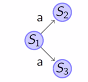
\includegraphics[width=.2\textwidth,keepaspectratio]{nfa_grafo_esempio}
    \caption{Grafo rappresentante un NFA}
    \label{nfa_grafo_esempio}
\end{figure}

\noindent Si noti anche che, nella rappresentazione grafica, gli archi da \(S_1\) a \(S_2\) ed \(S_3\) vengono denotati da \(a\).

Proponiamo ora al lettore il seguente esempio (figura \ref{nfa_grafo_2}):
\begin{figure}
    \centering
    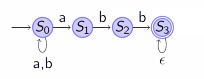
\includegraphics[width=.5\textwidth,keepaspectratio]{nfa_grafo_2}
    \caption{Secondo esempio di NFA}
    \label{nfa_grafo_2}
\end{figure}
L’elemento non deterministico è rappresentato dalle dure frecce \(a\) uscenti da \(S_0\), che potrebbero portarmi sia in \(S_1\) che in \(S_0\) di nuovo; inoltre, la \(\varepsilon\) introduce sempre indeterminismo, poiché permette di passare a uno stato successivo senza consumare un carattere del terminale (o produrre un carattere nella stringa, che dir si voglia), e quindi inserisce incertezza riguardo al percorso di derivazione compiuto.

Notiamo che dalla rappresentazione grafica si evincono tutti gli elementi che compongono l’NFA; questa è infatti una rappresentazione completa.
Si può anche dare una descrizione tabellare delle funzioni di transizione (\(\textrm{move}_n\)) appartenenti a questo NFA:

%TODO: sostituire con una tabella vera
\begin{figure}
    \centering
    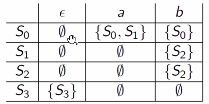
\includegraphics[width=.4\textwidth,keepaspectratio]{tabella}
    \caption{Tabella}
    \label{tabella}
\end{figure}

Qual è quindi il linguaggio accettato da un automa di questo tipo?\label{linguaggio_definito_da_un_automa} 
Un NFA \(\mathcal{N}\) accetta (o riconosce) una parola \(w\) se e solo se esiste almeno un cammino che parte dallo stato iniziale di \(\mathcal{N}\) ed arriva a \(w\).

Ricorda queste regole di scrittura:
\begin{itemize}
    \item \(\varepsilon \varepsilon\) si scrive \(\varepsilon\);
    \item \(a\varepsilon\) si scrive \(a\);
    \item \(\varepsilon a\) si scrive \(a\).
\end{itemize}

Il linguaggio accettato dall’automa è l’insieme di tutte le parole accettate dall’automa.
Risolviamo, ad esempio, il linguaggio generato dall’automa descritto in figura \ref{nfa_grafo_2}:
\begin{itemize}
    \item \(a\) non appartiene al linguaggio, non esiste un percorso che mi porti ad uno stato finale attraversando un solo arco \(a\);
    \item allo stesso modo non posso trovare la parola \(b\) nel linguaggio;
    \item una parola possibile in questo linguaggio è, ad esempio, \(abb\);
    \item tutte le parole nella forma \(\mathcal{L}(a \mid b)^\ast abb\) sono parte del linguaggio.
\end{itemize}

\noindent Proviamo a determinare il linguaggio dell'NFA descritto in figura \ref{nfa_grafo_3}:

\begin{figure}
    \centering
    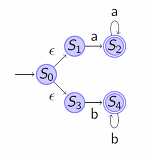
\includegraphics[width=.3\textwidth,keepaspectratio]{nfa_grafo_3}
    \caption{}
    \label{nfa_grafo_3}
\end{figure}

\noindent Il linguaggio accettato da questo NFA è \(\mathcal{L}((a a^* ) \mid ( b b^\ast ))\).

\section{La costruzione di Thompson}
La costruzione di Thompson è una procedura algoritmica che permette di costruire l’automa \(\mathcal{N}\) che genera lo stesso linguaggio denotato da una certa espressione regolare \(r\), ovvero \(\mathcal{L}(\mathcal{N}) = \mathcal{L}(r)\).

\subsection{Definizione}
Anche questa costruzione è espressa in modo induttivo.

\begin{description}
    \item[Base] L'espressione regolare \(r\) è o \(\varepsilon\), oppure un simbolo dell’alfabeto \(a \in \mathcal{A}\); assumiamo di avere sempre un NFA che riconosce \(\mathcal{L}(\varepsilon)\) e uno che riconosce \(\mathcal{L}(a) \; \forall a \in \mathcal{A}\).
    \item[Step] L'espressione regolare \(r\) è una tra le seguenti opzioni: 
    \begin{itemize}[noitemsep]
        \item \(r_1 \mid  r_2 \);
        \item \( r_1 r_2 \); 
        \item \( r_1\) \(^\ast \);
        \item \((r_1)\);
    \end{itemize}
    e, dati gli NFA \(\mathcal{N}_1\) e \(\mathcal{N}_2\) tali che \(\mathcal{L}(\mathcal{N}_1)=\mathcal{L}(r_1)\) e \(\mathcal{L}(\mathcal{N}_2) = \mathcal{L}(r_2)\), dobbiamo definire i vari NFA per le quattro operazioni \(r_1 \mid r_2\), \(r_1 r_2\), \(r_1\) \(^\ast\) ed \(r_1\). Le regole per definire questi nuovi NFA sono elencate successivamente.
\end{description}

\noindent A questo punto possiamo fare due osservazioni sulla costruzione di Thompson.

\begin{enumerate}
    \item Ogni passo della costruzione introduce al massimo due nuovi stati, vale a dire che l’NFA generato contiene al massimo \(2k\) stati, dove \(k\) è il numero di simboli e operatori nell’espressione regolare.
    \item In ogni stato intermedio dell’NFA c’è esattamente uno stato finale, e inoltre lo stato iniziale non ha nessun arco entrante e lo stato finale non ha alcun arco uscente. 
\end{enumerate}

\subsection{Spiegazione in dettaglio}
Vediamo ora la rappresentazione grafica di questo algoritmo. Partiamo dai passi base.

\begin{figure}
    \centering
    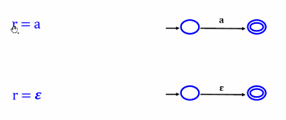
\includegraphics[width=.5\textwidth,keepaspectratio]{Thompson_base}
    \caption{Thompson per il caso base}
    \label{Thompson_base}
\end{figure}

\noindent La spiegazione dell'algoritmo nel caso base è banale, osserviamo invece con più interesse lo step induttivo.

\begin{figure}
    \centering
    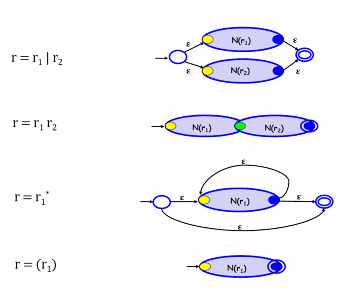
\includegraphics[width=.7\textwidth,keepaspectratio]{Thompson_step}
    \caption{Thompson per lo step iduttivo}
    \label{Thompson_step}
\end{figure}
Supponiamo di avere \(\mathcal{N}(r_1)\) e \(\mathcal{N}(r_2)\) descritti come in precedenza, discutiamo le applicazioni di Thompson descritte in in figura \ref{Thompson_step}.

\subsubsection{Alternation}
Guardiamo il primo caso, l'operazione di addizione \(r = r_1 \mid r_2\).\\
Vogliamo creare un automa che accetta parole di \(\mathcal{L}(r_1)\) o anche parole di \(\mathcal{L}(r_2)\).
Abbiamo i due \(\mathcal{N}\), che rappresentano gli stati intermedi; li posizioniamo uno sopra all’altro. Ora possiamo creare uno stato vuoto e usarlo come stato iniziale per entrambi gli \(\mathcal{N}\), e quindi collegarlo a questi ultimi tramite una \(\varepsilon\)-trasformazione; allo stesso modo possiamo creare uno stato finale raggiungibile dai due \(\mathcal{N}\) tramite una \(\varepsilon\)-trasformazione.

\subsubsection{Concatenation}
Guardiamo ora l’operazione di concatenazione \(r = r_1 r_2\).\\
Per la nostra ipotesi induttiva, sappiamo di poter far affidamento sui due automi \(\mathcal{N}(r_1)\) ed \(\mathcal{N}(r_2)\); in questo momento ci viene in aiuto la proprietà della costruzione, che dice che i passi intermedi (i due \(\mathcal{N}\)) hanno esattamente uno stato finale ed uno stato iniziale, senza alcun arco entranto nello stato iniziale e nessun arco uscente dagli stati finali. 
In questo modo possiamo far coincidere lo stato iniziale di \(\mathcal{N}(r_2)\) con lo stato finale di \(\mathcal{N}(r_1)\). 
Di conseguenza, una parola riesce ad arrivare allo stato terminale blu solo se riesce a passare sia da \(\mathcal{N}(r_1)\) che da \(\mathcal{N}(r_2)\).

\subsubsection{Kleene Star}
Guardiamo il caso della Kleene star \(r = r_1^*\).\\
Vogliamo un automa che riconosce o \(\varepsilon\) o tutte le parole che sono composte dalla ripetizione di altre parole appartenenti al linguaggio \(\mathcal{L}(r_1)\).
Posseggo l’automa \(\mathcal{N}(r_1)\), che ha un solo stato iniziale ed un solo stato finale; aggiungo due stati che serviranno come nuovo stato iniziale e nuovo stato finale.
Siccome voglio poter avere \(\varepsilon\) come parola possibile, introduco un nuovo arco \(\varepsilon\) che collega il nuovo stato iniziale al nuovo stato finale, quindi implemento la ripetizione con degli altri archi \(\varepsilon\) come in figura; la spiegazione è abbastanza banale.

\subsubsection{Parentheses}
Guardiamo il caso della parentesizzazione \(r = ( r_1 )\), il quale risulta estremamente banale, così tanto che in realtà non lo guardiamo davvero scherzone lol.

Questo è il modo di utilizzare il processo di Thompson per costruire automi complessi, ci renderemo conto più avanti di quante \(\varepsilon\) questo ci costringe ad utilizzare e di cosa questo comporti.

\subsection{Applicazione di Thompson}
Presentiamo ora un esempio particolare per assimilare meglio questa costruzione. Analizziamo il seguente linguaggio:

\begin{equation}
    r = (a \mid b)^\ast abb
\end{equation}

\noindent Ci sono quindi due espressioni che compaiono in questo esempio: \(a = r_1\) e \(b = r_2\).
In primis applichiamo la regola di base (\ref{Thompson_base}).

\begin{figure}
    \centering
    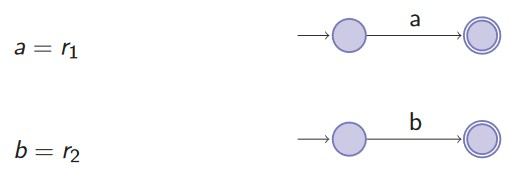
\includegraphics[width=.7\textwidth,keepaspectratio]{esempio_Thompson_0}
    \caption{Applicazione del passo base della costruzione di Thompson}
    \label{esempio_Thompson_0}
\end{figure}

Concentriamoci ora sulla prima espressione, \( a \mid b = r_1 \mid r_2 = r_3\); applichiamo la costruzione di Thompson per l’alternanza ai due automi per \(r_1\) e \(r_2\), otteniamo quindi l’automa per \(r_3\).

\begin{figure}
    \centering
    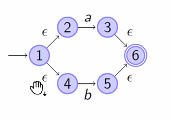
\includegraphics[width=.4\textwidth,keepaspectratio]{esempio_Thompson_1}
    \caption{Applicazione della costruzione per l'alternanza}
    \label{esempio_Thompson_1}
\end{figure}

La procedura è rappresentata in figura \ref{esempio_Thompson_1} ed è qui brevemente descritta: prendiamo i due automi per \(r_1\) ed \(r_2\), li mettiamo uno sopra l’altro e generiamo due stati (nodo \(1\) e nodo \(6\)); il nodo \(1\) sarà collegato tramite archi \(\varepsilon\) agli stati iniziali di entrambi gli automi, e simmetricamente il nodo \(6\) verrà collegato tramite archi \(\varepsilon\) agli stati finali dei due automi.

Il prossimo passaggio è la traduzione dell'operatore di parentesi, il che è banale, quindi ne riportiamo solo una formulazione nel linguaggio delle espressioni regolari:

\begin{equation*}
    (a \mid b)=(r_3)=r_4
\end{equation*}

\noindent Ora dobbiamo rappresentare la seguente espressione:

\begin{equation*}
    (a\mid b)^\ast = r_4^\ast = r_5
\end{equation*}

\noindent Quindi applichiamo la costruzione di Thompson per la Kleene star all’automa per \(r_4\), ottenendo quindi l’automa per \(r_5\).

\begin{figure}
    \centering
    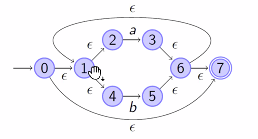
\includegraphics[width=.5\textwidth,keepaspectratio]{esempio_Thompson_2}
    \caption{Applicazione della costruzione per la Kleene star}
    \label{esempio_Thompson_2}
\end{figure}

\noindent Continuando con la scansione dell’espressione regolare dobbiamo riscrivere la seguente:

\begin{equation}
    (a \mid b)^\ast a = r_5 r_1 = r_6
\end{equation}

\noindent Applichiamo quindi la costruzione di Thompson per la concatenazione.

\begin{figure}
    \centering
    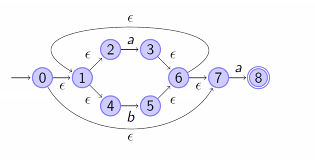
\includegraphics[width=.5\textwidth,keepaspectratio]{esempio_Thompson_3}
    \caption{Applicazione della costruzione per la concatenazione}
    \label{esempio_Thompson_3}
\end{figure}

\noindent Dobbiamo infine riapplicare il passo della concatenazione per le due \(b\) mancanti.

\begin{figure}
    \centering
    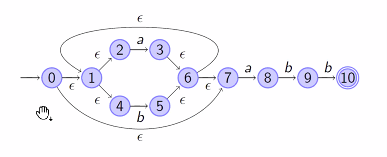
\includegraphics[width=.5\textwidth,keepaspectratio]{esempio_Thompson_4}
    \caption{Applicazione della costruzione per la concatenazione (II)}
    \label{esempio_Thompson_4}
\end{figure}

Possiamo notare come il risultato cui giungiamo sia pieno di \(\varepsilon\); la costruzione di Thompson ci dà sicuramente un risultato esatto, ma non è detto che sia il risultato migliore, anzi; abbiamo già visto in passato un automa che riconosce lo stesso linguaggio di questo, e quell'automa era più semplice ed elegante (vedi \ref{nfa_grafo_2}).

Notiamo che comunque l’algoritmo di Thompson garantisce dei limiti superiori sulla complessità dell’automa che genera: ad ogni passo si aggiungono al massimo \(2\) nuovi nodi.
La lunghezza dell’automa finale infatti è limitata da \(2n\), con \(n\) che rappresenta il numero di simboli nell’espressione regolare, dove con simboli si intende sia simboli del vocabolario che operatori.

Anche il numero di archi è limitato in quanto per ogni passaggio si aggiungono al massimo \(4\) archi.

\section{Il processo di simulazione dell’automa}
Le nostre conoscenze attuali ci permettono di costruire un automa per una certa espressione regolare, ma come si fa a decidere se una certa parola \(w\) fa parte del linguaggio di un dato automa \(\mathcal{N}\)? Si utilizza una procedura detta \emph{simulazione dell’automa}.

Abbiamo già definito in \ref{linguaggio_definito_da_un_automa} come viene deciso se una parola fa parte del linguaggio riconosciuto dall’automa; prendiamo ora ad esempio \(w = bbb\) e l’automa presentato in figura \ref{automa_secondo_esempio}, e presentiamo la procedura di simualzione di un automa.

\begin{figure}
    \centering
    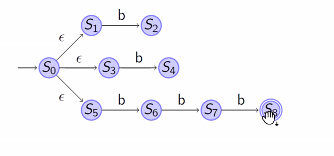
\includegraphics[width=.6\textwidth,keepaspectratio]{automa_secondo_esempio}
    \caption{Esempio di automa}
    \label{automa_secondo_esempio}
\end{figure}

Se dovessimo fare “a occhio”, questo caso sarebbe molto semplice da risolvere: si parte dallo stato \(S_0\) e si va in un altro stato tramite o archi \(\varepsilon\) o tramite archi \(b\); una volta che raggiungo uno stato con un arco \(b\) elimino il primo carattere della parola e procedo con il secondo, cerco archi con \(\varepsilon\) o con il secondo carattere e così via.
La parola appartiene al linguaggio riconosciuto dall’automa se consumo l’ultimo carattere della parola in uno stato finale.

Noi però stiamo cercando un algoritmo formale che faccia queste operazioni, e che le faccia senza necessità di backtrack per tornare indietro se un percorso si rivela errato, operazione altamente costosa.
Cosa possiamo fare per velocizzare il processo?

Vediamo che leggere \(bbb\) da \(S_0\) è uguale a leggerlo da uno qualunque tra gli stati \(\{S_0, S_1, S_3, S_5\}\), perché arrivo a questi stati solo tramite archi \(\varepsilon\); non potremmo quindi semplificare tutti questi in un solo nodo?

La risposta è sì, possiamo farlo! Per vedere in che modo dobbiamo prima introdurre il concetto di \(\varepsilon\)-chiusura.


\subsection{\(\varepsilon\)-chiusura di un automa}
Sia \((S, \mathcal{A}, \textrm{move}_n, s_0, F)\) un NFA, sia \(t\) uno stato in \(S\) e \(T\) un sottoinsieme di \(S\).

Definiamo \(\varepsilon\)-chiusura\((\{t\})\) l’insieme di stati in \(S\) che sono raggiungibili da \(t\) tramite zero o più \(\varepsilon\)-transizioni (nota che \(t\) è sempre in questo insieme).

Definiamo \(\varepsilon\)-chiusura\((T)\) nel seguente modo:
\begin{equation}
    \varepsilon \textrm{-chiusura}(T) = \bigcup_{t \in T} \;\varepsilon\textrm{-chiusura}(\{t\})
\end{equation} 

\subsubsection{Calcolo della \(\varepsilon\)-chiusura}
Per calcolare la \(\varepsilon\)-chiusura di un nodo di un automa useremo queste strutture:

\begin{enumerate}
    \item Uno stack;
    \item Un array booleano “alreadyOn” che ci serve per segnalare se uno stato \(t\) è già sulla pila o meno (la sua lunghezza è \(|S|\));
    \item Un array bidimensionale per ricordare \(\textrm{move}_n\). Ogni entry \((t,x)\) è una lista linkata contenente tutti gli stati che sono raggiungibili con un \(x\)-transizione da \(t\).
\end{enumerate}

Ora che sappiamo quali sono le strutture dati che andremo ad utilizzare, studiamo la fase di inizializzazione: 

\begin{itemize}
    \item all’inizio dei tempi non c’è niente sulla pila, poi inseriamo \(t\) e lo segnaliamo su alreadyOn;
    \item a questo punto estraiamo dalla cima dello stak, prendiamo il nodo estratto \(e\) e cerchiamo tutti i nodi che da \(e\) si raggiugono tramite un \(\varepsilon\)-arco; inseriamo tutti questi nello stak (se non sono già presenti) e ne segnaliamo l'inserimento settando il loro flag su alreadyOn.
\end{itemize}

Continuiamo così finché lo stak non si svuota. L'algoritmo appena descritto si può trovare in figura \ref{algoritmo_epsilon_chiusura}.

\begin{figure}[H]
    \centering
    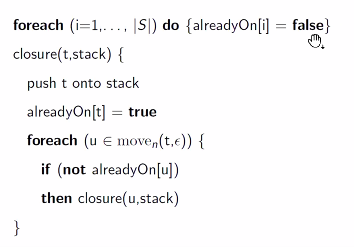
\includegraphics[width=.6\textwidth,keepaspectratio]{algoritmo_epsilon_chiusura}
    \caption{Algoritmo per il calcolo della \(\varepsilon\)-chiusura\((\{t\})\)}
    \label{algoritmo_epsilon_chiusura}
\end{figure}

% \begin{algorithm}[H]
% 	\centering
	\subimport{assets/code/}{epsilon-closure-computation.tex}
	% \caption{Esempio di parse tree}
% \end{algorithm}

Ora che abbiamo l'arma della \(\varepsilon\)-chiusura possiamo procedere con l'algoritmo per la verifica dell'appartenenza di una parola \(w\) al linguaggio riconosciuto da un automa, ovvero l'algoritmo di simulazione (figura \ref{algoritmo_simulazione_nfa}).

\begin{figure}
    \centering
    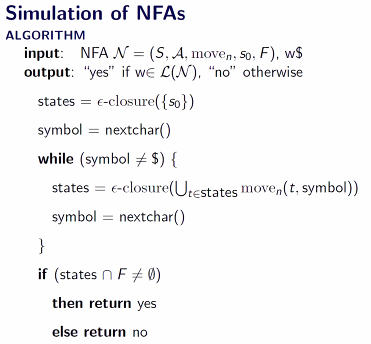
\includegraphics[width=.6\textwidth,keepaspectratio]{algoritmo_simulazione_nfa}
    \caption{Algoritmo di simulazione per un automa}
    \label{algoritmo_simulazione_nfa}
\end{figure}

Dove \texttt{\$} è l’end-marker per la parola \(w\) (alcuni testi usano la “gratella” invece che \texttt{\$}).
Il funzionamento dell'algoritmo è questo: calcoliamo la \(\varepsilon\)-chiusura di \(s_0\) e la aggiungiamo all'insieme \texttt{states}; prendiamo il primo simbolo nella parola e poi entriamo nel ciclo che compone il corpo della procedura.

In questo corpo si utilizza la \(\varepsilon\)-chiusura per salvare in \texttt{states} la \(\varepsilon\)-chiusura di tutti gli stati che posso raggiungere tramite una \texttt{symbol}-transizione (una transizione marcata con \texttt{symbol}); una volta trovati questi nodi passo \texttt{symbol} prende il valore del prossimo carattere di \(w\).

Una volta che \texttt{symbol} prende il valore di \texttt{\$}, mi fermo e controllo il contenuto di \texttt{states}.

Se \(\textrm{\texttt{states}} \; \cap \; F \neq \Phi\), allora significa che esiste uno stato in \texttt{states} che è anche uno stato finale dell'automa e quindi abbiamo trovato un percorso che riconosce la parola \(w\) e termina in uno stato finale (ammissibile). Ottimo, abbiamo appena dimostrato che \(w\) appartiene al linguaggio riconosciuto dall'automa.

Se invece la condizione precedente non è verificata, allora si è avverato uno dei seguenti casi (o anche entrambi): o non esistono percorsi che riconoscono \(w\), o non esistono percorsi che riconoscono \(w\) e terminano in uno stato finale.

\subsection{Esempi di simulazione}
Applichiamo ora, come esempio, l'algoritmo di simulazione di un NFA dato, verificando se accetta la parola \(w  = ababb\). Lo svolgimento è rappresentato in figura \ref{simulazione_es_1}.

\begin{figure}
    \centering
    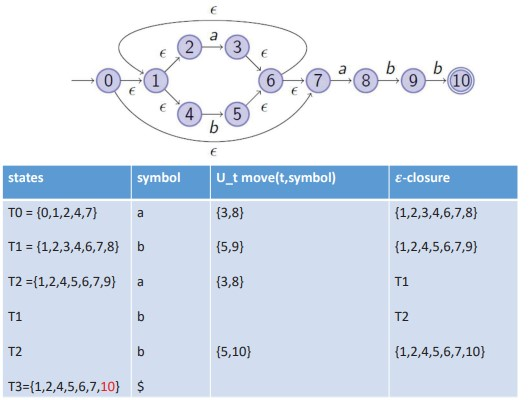
\includegraphics[width=.6\textwidth,keepaspectratio]{simulazione_es_1}
    \caption{Esempio di applicazione dell'algoritmo di simulazione}
    \label{simulazione_es_1}
\end{figure}

\noindent In seguito una breve descrizione della rappresentazione dell'algoritmo.

Inizializziamo la variabile \texttt{states} a \(T0\) inserendo la \(\varepsilon\)-chiusura di \(0\); poi estraiamo il simbolo da aggiungere (il primo simbolo di \(w\)) che è \(a\).

Ora devo comporre l’insieme di stati che posso raggiungere da \texttt{states} con una \(a\)-transizione, e questo insieme è \(\{3, 8\}\). 

Di questo insieme l’algoritmo dice che devo calcolare la \(\varepsilon\)-chiusura, che corrisponde all’insieme nell’ultima colonna della prima riga; questo è il mio nuovo insieme di stati \(T1\) da cui partirò nello step successivo.

Nel secondo step il simbolo che devo aggiungere è la seconda lettera di \(w\), ovvero \(b\), quindi vado a cercare quei nodi che posso raggiungere da \(T1\) con una \(b\)-transizione; questi nodi sono \(\{5,9\}\), e una volta che li ho trovati ne calcolo la \(\varepsilon\)-chiusura, che compone \(T2\) e via così.

Continuo così finché non finisco i simboli; a quel punto devo verificare se esiste nel mio insieme \(states\) uno stato finale. In questo caso è presente (\(10\)), e quindi la parola \(w\) appartiene al linguaggio riconosciuto dall’automa raffigurato.


\subsection{Nota sulla \(\varepsilon\)-chiusura}
\begin{theorem}
    Sia \((S, \mathcal{A}, \textrm{move}_n, s_0, F)\) un NFA e sia \(M \subseteq S\).
    
    Allora la \(\varepsilon\)-chiusura\((M)\) è il più piccolo insieme \(X \subseteq S\) tale che \(X\) è una soluzione alla seguene equazione:
    \begin{equation}
        X = M \cup \{ N’ \mid N \in X \land N’ \in \textrm{move}_n (N,\varepsilon)\}
    \end{equation}
\end{theorem}

\noindent Nota che diciamo il più piccolo insieme per evitare di proseguire in loop infiniti come quello rappresentato in figura \ref{nfa_ciclico}.

\begin{figure}
    \centering
    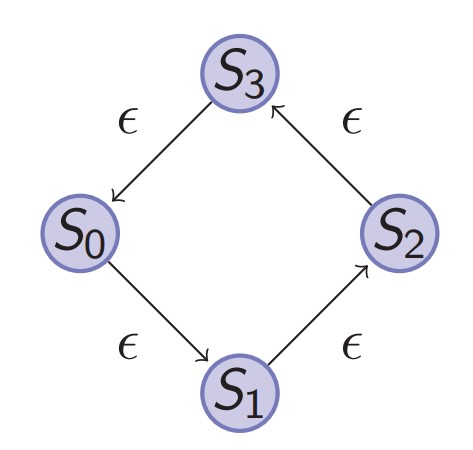
\includegraphics[width=.3\textwidth,keepaspectratio]{nfa_ciclico}
    \caption{Se non scegliessimo il più piccolo \(X\) potremmo incorrere in cicli infiniti.}
    \label{nfa_ciclico}
\end{figure}

Osserviamo con attenzione la formula appena descritta: \(X\) è \(M\) stesso, unito anche a tutti gli stati \(N’\) raggiungibili da \(N\) tramite una \(\varepsilon\)-transizione, dove \(N\) è uno stato qualsiasi in \(M\).

Balza subito all'occhio come la formula per definire \(X\) dipenda da \(X\) stessa; per questo motivo non dovremmo poterla calcolare, giusto? 
Sbagliato! In informatica possiamo risolvere queste equazioni date certe caratteristiche, ed è qui che giunge in nostro aiuto il teorema del punto fisso.


\subsection{Teorema del punto fisso}
\begin{theorem}
    Sia \(f: 2^S \to 2^S\) per qualche insieme finito \(D\), sia inoltre \( f \) monotona (ovvero \(X \subseteq Y \implies f(X) \subseteq f(Y)\)).

    Allora esiste una precisa tecnica per risolvere l'equazione \(X = f(X)\).
\end{theorem}



\end{document}